\documentclass{article}
\usepackage[utf8x]{inputenc}
\usepackage{ucs}
\usepackage{amsmath} 
\usepackage{amsfonts}
\usepackage{upgreek}
\usepackage[english,russian]{babel}
\usepackage{graphicx}
\usepackage{float}
\usepackage{textcomp}
\usepackage{hyperref}
\usepackage{geometry}
  \geometry{left=2cm}
  \geometry{right=1.5cm}
  \geometry{top=1cm}
  \geometry{bottom=2cm}
\usepackage{tikz}
\usepackage{ccaption}
\usepackage{multicol}

\usepackage{listings}
%\setlength{\columnsep}{1.5cm}
%\setlength{\columnseprule}{0.2pt}


\begin{document}
\pagenumbering{gobble}

\lstset{
  language=C,                % choose the language of the code
  basicstyle=\linespread{1.1}\ttfamily,
  columns=fixed,
  fontadjust=true,
  basewidth=0.5em,
  keywordstyle=\color{blue}\bfseries,
  commentstyle=\color{gray},
  stringstyle=\ttfamily\color{orange!50!black},
  showstringspaces=false,
  %numbers=false,                   % where to put the line-numbers
  numbersep=5pt,
  numberstyle=\tiny\color{black},
  numberfirstline=true,
  stepnumber=1,                   % the step between two line-numbers.        
  numbersep=10pt,                  % how far the line-numbers are from the code
  backgroundcolor=\color{white},  % choose the background color. You must add \usepackage{color}
  showstringspaces=false,         % underline spaces within strings
  captionpos=b,                   % sets the caption-position to bottom
  breaklines=true,                % sets automatic line breaking
  breakatwhitespace=true,         % sets if automatic breaks should only happen at whitespace
  xleftmargin=.2in,
  extendedchars=\true,
  keepspaces = true,
}
\lstset{literate=%
   *{0}{{{\color{red!20!violet}0}}}1
    {1}{{{\color{red!20!violet}1}}}1
    {2}{{{\color{red!20!violet}2}}}1
    {3}{{{\color{red!20!violet}3}}}1
    {4}{{{\color{red!20!violet}4}}}1
    {5}{{{\color{red!20!violet}5}}}1
    {6}{{{\color{red!20!violet}6}}}1
    {7}{{{\color{red!20!violet}7}}}1
    {8}{{{\color{red!20!violet}8}}}1
    {9}{{{\color{red!20!violet}9}}}1
}

\title{Семинар \#4: Типы данных. \vspace{-5ex}}\date{}\maketitle
\section*{Часть 1: Целочисленные типы данных.}
Различные целочисленные типы языка C представлены в следующей таблице:

\begin{center}
\begin{tabular}{ c c c c }
 тип & размер (байт) & диапазон значений ($2^{\# bits}$) & спецификатор \\ \hline
 char & 1 & от -128 до 127 & \texttt{\%hhi} \\ 
 short & 2 & от -32768 до 32767 & \texttt{\%hi}  \\  
 int & 4 & примерно от -2-х миллиардов до 2-х миллиардов & \texttt{\%i}  \\  
 long & 4 или 8 & такой же как у int или long long в зависимости от системы & \texttt{\%li}  \\  
 long long & 8 & примерно от $-10^{19}$ до $10^{19}$ & \texttt{\%lli}  \\  
 unsigned char & 1 & от 0 до 255 & \texttt{\%hhu} \\ 
 unsigned short & 2 & от 0 до 65535 & \texttt{\%hu}  \\  
 unsigned int & 4 & примерно от 0 до 4-х миллиардов & \texttt{\%u}  \\  
 unsigned long & 4 или 8 & такой же как у unsigned int или unsigned long long & \texttt{\%lu}  \\  
 unsigned long long & 8 & от 0 до $2^{64} \approx 2*10^{19}$  & \texttt{\%llu}  \\  
 size\_t & 4 & примерно от 0 до 4-х миллиардов & \texttt{\%zu} \\ \hline 
\end{tabular}
\end{center}
Это наиболее распространённые значения размеров типов для 64-х битных систем, но на некоторых системах эти значения могут быть другими.
Чтобы узнать эти значения можно использовать оператор \texttt{sizeof}. \\

\section*{Часть 2: Новое имя типа}
В языке C существует возможность вводить новое имя для уже существующего типа с помощью ключевого слова \texttt{typedef}. Чтобы ввести новое имя для типа нужно написать следующее:
\begin{lstlisting}
typedef староеимя новоеимя;
\end{lstlisting}
После этого для типа можно будет использовать и новое и старое имя.


\subsection*{Тип \texttt{size\_t}} 
Тип \texttt{size\_t} -- это беззнаковый тип целых чисел, который выбирается таким образом, чтобы он вмещал размер любого массива. Внутри стандартной библиотеки может быть написано примерно следующее:
\begin{lstlisting}
typedef unsigned long long size_t;
\end{lstlisting}
Но размер типа \texttt{size\_t} может различаться в зависимости от вычислительно системы. Выясните чему он равен на вашей системе.

\newpage
\section*{Часть 3: Числа с плавающей точкой. Библиотека \texttt{math.h}}
\begin{center}
\begin{tabular}{ c c c c c }
 тип & размер (байт) & значимые цифры & диапазон экспоненты & спецификатор \\ \hline
 float             & 4          & 6  & от -38 до 38    & \texttt{\%f} \\ 
 double            & 8          & 15 & от -308 до 308  & \texttt{\%lf}  \\  
 long double       & от 8 до 16 & $\ge 15$  & не хуже чем у double  & \texttt{\%Lf}  \\ \hline
 печать только 3-х чисел после запятой & -          & -  & -              & \texttt{\%.3f} \\
 печать без нулей на конце & -          & -  & -              & \texttt{\%g} \\
 печать в научной записи   & -          & -  & -              & \texttt{\%e} \\
\end{tabular}
\end{center}


\subsection*{Библиотека \texttt{math.h}}
В библиотеке \texttt{math.h} содержатся множество полезных математических функций.

\begin{center}
\begin{tabular}{ c c }
 функция & что делает \\ \hline
 \texttt{sqrt}     & Вычисляет корень числа \\ 
 \texttt{abs}      & Вычисляет модуль целого числа \\ 
 \texttt{fabs}     & Вычисляет модуль числа с плавающей точкой \\ 
 \texttt{exp}      & Экспонента $e^x$ \\ 
 \texttt{log}      & Натуральный логарифм $ln(x)$ \\
 \texttt{sin}, \texttt{cos},  \texttt{tan} & Синус, косинус и тангенс (радианы) \\ 
 \texttt{asin}, \texttt{acos},  \texttt{atan} & Арксинус, арккосинус и арктангенс \\ 
 \texttt{floor}      & Округление до ближайшего меньшего целого числа \\
 \texttt{ceil}       & Округление до ближайшего большего целого числа \\
 \texttt{pow(x, y)}        & Возведение числа в \texttt{x} степень \texttt{y} \\
\end{tabular}
\end{center}


\subsection*{Точность чисел с плавающей точкой}
Количество вещественных чисел на любом отрезке бесконечно, а количество возможных значений чисел с плавающей точкой ограничено, поэтому не каждое вещественное число можно закодировать числом \texttt{float} или \texttt{double}. Это означает, что числа с плавающей точкой всегда вычисляются с погрешностью. Поэтому сравнивать 2 таких числа оператором сравнения \texttt{==} очень опасно. Например, следующая программа напечатает \texttt{No}.
\begin{lstlisting}
#include <stdio.h>
int main() 
{
    float a = 3 * 0.1;
    float b = 0.3;
    if (a == b)
        printf("Yes\n");
    else
        printf("No\n");
}
\end{lstlisting}

Такие числа всегда нужно сравнивать с некоторой точностью $\epsilon$ по формуле $|a - b| < \epsilon$. Вот так:\\ 
\begin{lstlisting}
#include <stdio.h>
#include <math.h>
int main() 
{
    float eps = 1e-5;
    float a = 3 * 0.1;
    float b = 0.3;
    if (fabs(a - b) < eps)
        printf("Yes\n");
    else
        printf("No\n");
}
\end{lstlisting}


\newpage
\section*{Часть 4: Указатели.}
Для хранения адресов в языке C введены специальные переменные, которые называются указатели. Тип переменной указателя = тип той переменной, чей адрес он хранит + звёздочка на конце. Например, указатель, который будет хранить адреса переменных типа \texttt{int} должен иметь тип \texttt{int*}. \\

\begin{center}
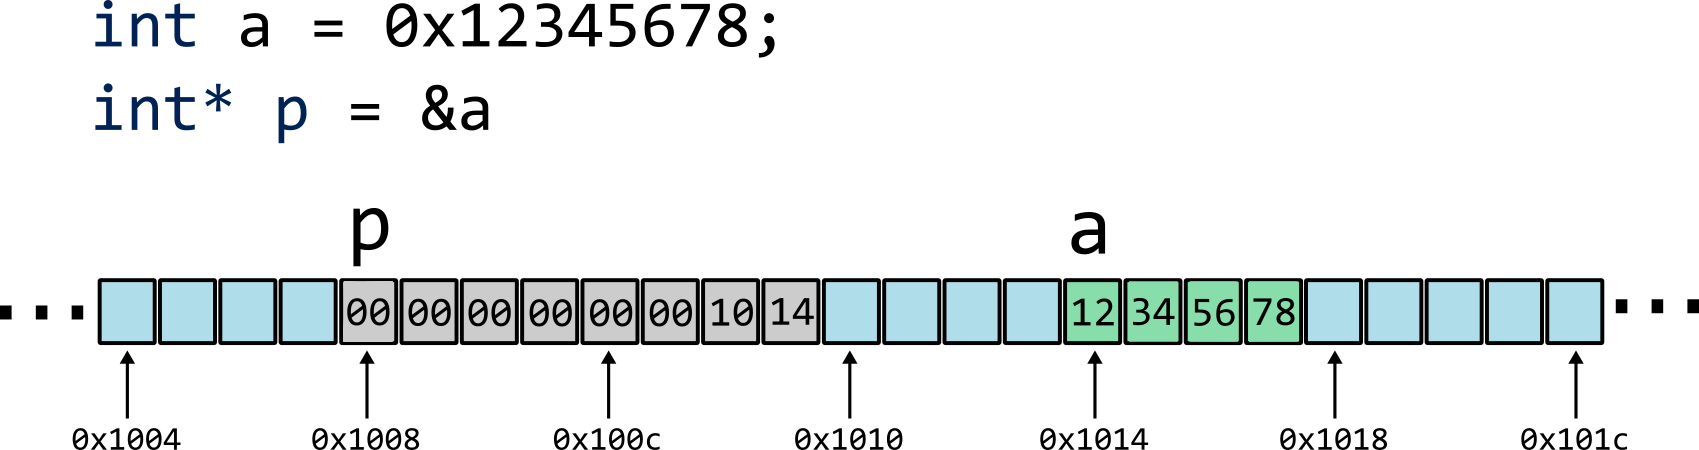
\includegraphics[scale=1]{../images/memory_3_pointer_to_int_b.png}
\end{center}
Пояснения по рисунку:
\begin{itemize}
\item Числа, начинающиеся с \texttt{0x} -- это числа в шестнадцатеричной записи.
\item В данном примере для простоты выбраны очень маленькие адреса. В действительности же адрес скорей всего будет очень большим числом.
\item Указатель тоже является переменной и хранится в памяти.
\item Указатель хранит номер одной из ячеек памяти (в данном случае -- первый байт \texttt{a}).
\end{itemize}

\subsection*{Операция разыменования:}
Разыменования -- это получение самой переменной по указателю на неё. Чтобы разыменовать указатель нужно перед ним поставить звёздочку. Не следует путать эту звёздочку со звёздочкой, используемой при объявлении указателя. То есть, если \texttt{p} это указатель, хранящий адрес \texttt{a}, то \texttt{*p} означает следующее:\\

\textit{Пройди по адресу, хранящемуся в \texttt{p}. Возьми соответствующее количество байт, начиная с этого адреса (в данном случае 4, так как \texttt{p} указывает на \texttt{int}). Воспринимай эти байты как переменную соответствующего типа (в данном случа \texttt{int}).}

\begin{lstlisting}
#include <stdio.h>
int main() 
{
    int a = 10;
    int* p = &a;
    *p += 1;
    printf("%d\n", a);
}
\end{lstlisting}

\newpage
\subsection*{Арифметика указателей}
С указателями можно производить следующие операции:
\begin{itemize}
\item Разыменование \texttt{*p}
\item Инкремент \texttt{p++}. В этом случае указатель не увеличивается на \texttt{1}, как было можно подумать. Он увеличивается на размер типа, на который он указывает. Благодаря этой особенности указателей с их помощью удобно проходить по массиву.
\item Декремент \texttt{p++}. Уменьшается на размер типа, на который он указывает.
\item Прибавить или отнять число \texttt{p + k}. В этом случае указатель не увеличивается на \texttt{k}, как было можно подумать. Он увеличивается на \texttt{k * sizeof(*p)}. Благодаря этой особенности указателей с их помощью удобно проходить по массиву. Если \texttt{p} указывает на \texttt{i}-ый элемент массива, то \texttt{p + 1} будет указывать на \texttt{i + 1} элемент массива.
\item Вычитать 2 указателя \texttt{p - q}. Вернётся разница между указателями делённая на размер типа указателя.
\item Квадратные скобки (прибавить число + разыменование): \quad \texttt{p[i] == *(p+i)}
\end{itemize}

\subsection*{Передача по указателю}
Передавая в функцию не саму переменную, а указатель на эту переменную, мы можем менять саму переменную внутри, используя указатель.
\begin{lstlisting}
#include <stdio.h>

void inc(int* p)
{
    *p += 1;
}

int main()
{
    int a = 10;
    inc(&a);
    printf("%i\n", a);
}
\end{lstlisting}

При передаче в функцию массива, туда на самом деле передаётся указатель на первый элемент этого массива.

\end{document}